%  SingleXBs
%  Created by Dave Williams on 2009-06-25.
%  

% header (fold)
\documentclass[]{article}

\usepackage{fancyhdr}
\usepackage{graphicx}
\usepackage[utf8]{inputenc}
\usepackage[round,numbers,sort&compress]{natbib} 
\addtolength{\parskip}{\baselineskip}
\setlength{\parindent}{0in}

\newcommand{\de}{$^\circ$~} % \ensuremath kills latex2png

% Allow setting of H in float placement
%\usepackage{float}
% Double or 1.5 space text
%\usepackage{setspace}
% Multi-part figures
%\usepackage{subfigure}
% Package for including code in the document
%\usepackage{listings}

\title{A multidimensional actomyosin cross-bridge model simulates radial forces and the effects of changes in sarcomere lattice spacing} 
\author{C.D.\ Williams, M.\ Regnier, T.L.\ Daniel}
\date{2009--06--25}
% header (end)

\begin{document}

\maketitle{}

\begin{abstract} 
The force muscle generates on activation, in directions both aligned with the contractile filaments and perpendicular to the contractile filaments, depends on the radial distance from one contractile filament to another. 
Existing mechanochemical models of muscle contraction treat myosin as a simple linear spring oriented parallel to the direction of the contractile filaments.
Here we describe a more complex myosin cross-bridge model that replicates myosin's force-generating power stroke by incorporating multiple springs. 
This model is based on the protein structure of myosin so that the four springs which comprise it correspond to mechanically relevant portions of myosin's structure, enabling monitoring of phenomena not possible with a single-spring cross-bridge.
The behavior of this four spring cross-bridge (4sXB) model is based on stochastic binding and distortion dynamics which are consequences of thermal fluctuations.  
This 4sXB obtains most parameters from published experimental measurements.

Radial force (force orthogonal to the direction of contraction) is generated by the 4sXB model's lever-arm during its power stroke in a mechanism similar to that seen in an \emph{in vivo} cross-bridge. 
Additionally, as occurs \emph{in vivo}, our 4sXB model has binding, state-transition kinetics, and temporal dynamics of force production that all vary with lattice spacing. 
The dependence of a cross-bridge's force production on lattice spacing follows from lattice spacing's influence over the angles of cross-bridge attachment and the distances which cross-bridges must extend over to bind. 
Additionally, we describe a simpler two spring cross-bridge (2sXB) model which replicates most of the 4sXB model's qualities. 
Unlike the 4sXB model, the length and angle of the springs constituting the 2sXB model can be determined analytically for any chosen head position without the use of iterative techniques, making it more computationally efficient.
The forces generated by both of these multi-spring cross-bridge models are similar. 
We show that the rate at which the multi-spring cross-bridges bind and generate force decreases as lattice spacing grows. 
The axial and radial forces generated by the multi-spring cross-bridge models increase in magnitude as lattice spacing is offset from the myosin head resting position. 
The isolated multiple-spring cross-bridge models experience variations in binding site location and lattice spacing which mirror those that can occur in intact muscle.
The isolated cross-bridge models' response to these changes in binding site location and lattice spacing mirror changes in intact, contracting muscle's force production. 
\end{abstract}

Keywords: myosin; spatially-explicit model; cross-bridge kinetics; lattice spacing; radial force; stochastic model % While this is not a spatially explicit model, it is targeted to use in one and as such will be of interest to those who are interested in such models.

\paragraph*{Author Summary} % (fold)
Models of muscle contraction have long treated the molecular motor myosin as a simple spring oriented parallel to its direction of movement. 
This assumption does not allow for prediction of the forces observed during muscle shortening, or for a description of the relationship between the maximum force produced and the spacing between contractile filaments. 
We develop an alternative model, still computationally efficient enough to be used in simulations of the sarcomere, that incorporates both linear and torsional (angle dependent, like those found in a watch) springs. 
This new type of model captures much of the behavior missing from single spring models of the cross-bridge.
% paragraph author_summary (end)

%TODO : Create a list of symbols. See where and if Biophysical J lets them be inserted.

\section*{Introduction} %(fold)

Radial forces are of the same order as axial forces in contracting muscles \citep{Cecchi1990, Millman1998}. 
These forces, along with radial lattice spacing, are thought to be a key determinant of muscle force generation \citep{Fuchs2005}. 
At the same time, structural information about myosin cross-bridges suggests that force is generated through the action of a lever arm \citep{Rayment1993, Uyeda1996, Huxley2000}.
That lever arm generates the strain accompanying the power stroke via a change in the rest angle at which the lever is attached to S1 region \citep{Huxley2000, Houdusse2001}. 
This change in angle occurs at the converter region, a flexible area which acts as a torsional or angular spring. 
It has been suggested these phenomena are related, that the radial forces a cross-bridge generates are a result of the lever arm's geometry \citep{Schoenberg1980b}. 

Existing theoretical and computational models of cross-bridge force generation, at the level of myofilaments, assume force is generated by a simple linear spring oriented parallel to the long axis of the myofilaments (Fig.~\ref{fig_xb_types}B).  % FIXME : Cite the kinetics subfigure first or switch it to be on the bottom of Figure 1.
This assumption has persisted from the earliest fundamental models of muscle contraction to more elaborate and spatially explicit models \citep{Huxley1957, Daniel1998, Chase2004, Tanner2007, Campbell2009}.  

In these prior models of muscle contraction, radial forces have been given less attention. 
As a result, geometries of the single spring cross-bridge models have changed little while kinetic schemes governing transitions between conformational states have increased in complexity \citep{Huxley1957, Pate1989, Daniel1998, Smith2008a}. % TODO : Are there more kinetics papers out there? 
To analyze the radial forces that occur during muscle contraction, a different cross-bridge geometry is needed: a geometry that produces both forces aligned with and forces orthogonal to the direction of contraction. 
A lever arm made of several springs can simulate the deformations a cross-bridge undergoes as it generates force (the power stroke), can provide a geometry which is usable in cross-bridge models, and can account for both axial and radial forces \citep{Houdusse2001}.  

In this paper we detail two models of cross-bridges that use multiple springs to replicate the lever arm mechanism.  
Both are sensitive to changes in lattice spacing and both account for the radial component of force produced during the power stroke.  
The first model (referred to as the 4sXB model) simulates the cross-bridge as a system of four linearly elastic springs arranged in a geometry based upon the structure of the S1 and S2 regions of myosin II (Fig.~\ref{fig_xb_types}D).  
Our second model (referred to as the 2sXB model) consists of two linearly elastic springs and provides greater computational efficiency than the 4sXB model while replicating many of the more complex model's behaviors (Fig.~\ref{fig_xb_types}C). 
Both the 4sXB model and the 2sXB model use a three-state model of the cross-bridge cycle's kinetics, consisting of an unbound state, a low-force pre-power stroke state, and a force-producing post-power stroke state. 
The kinetics of transition from one state to another in our models are similar to those used previously but are generalized for use in two dimensions; our kinetics calculate transition probabilities using the free energy landscape of the cross-bridges instead of the offset of the cross-bridge head (Fig.~\ref{fig_xb_types}A) \citep{Pate1989, Daniel1998, Tanner2007}. 
We quantify both axial and the radial forces produced by our two cross-bridge models. 
Additionally, we explain how changes in lattice spacing affect kinetics and forces in our multiple-spring models. 
% section introduction (end)


\section*{Methods}  % (fold)

Our two cross-bridge models, the 4sXB and the 2sXB (Figs.~\ref{fig_xb_types}C-D), are designed to capture a range of mechanical behaviors suggested by the literature, namely radial force generation and tuning of force-generated lattice spacing changes.  
Both are based on an arrangement of linearly elastic torsional, or angular, and Hookean springs.  

\subsection*{Geometry} % (fold)

\paragraph{Spring configurations} % (fold)
For comparison to previous models, we employ a simple cross-bridge model consisting of a linearly elastic spring oriented parallel to the long axis of the thick filament (1sXB, Fig.~\ref{fig_xb_types}B).  
Forces generated by this cross-bridge are oriented solely in the direction of shortening (axially oriented). 
This 1sXB model is identical to those used in recent spatially-explicit computational analyses \citep{Daniel1998, Chase2004, Tanner2007}. 
By definition, the one-dimensional 1sXB model cannot yield radial forces.  
Moreover, this model's geometry cannot account for lattice spacing dependent forces or kinetics.

The four-spring cross-bridge model, uses two linear and two torsional springs to represent the myosin head (Fig.~\ref{fig_xb_types}D).
This arrangement of springs closely corresponds to regions of the cross-bridge that are thought to regulate and respond to strain or deformation. 
In particular, the four springs correspond to the point where the S2 region attaches to the rod, or $\alpha$; the S2 region, or $\beta$; the point where the S2 region attaches to the light chain domain (LCD), or $\delta$; and the LCD, or $\gamma$ (Fig.~\ref{fig_xb_types}D, Table~\ref{parameter_table}). 
The torsional spring $\delta$ generates the force of the power stroke by a change in rest angle, mimicking myosin's force generation by lever-arm \citep{Houdusse2000, Houdusse2001}. 
Since the angle at which the head attaches to actin remains unchanged in our model, the torque generated at the converter region can be accounted for in a torsional spring on the end of LCD linear spring closer to the thick filament attachment point \citep{Houdusse2000}. 
The 4sXB model, by using multiple springs and existing in two dimensions,  allows us to compute radial forces and other cross-bridge properties that are not present in the 1sXB's one-dimensional space. 
The rest angle of the torsional spring linking the S2 domain and the LCD simulates the power stroke by increasing during the transition from a pre-power stroke to a post-power stroke state.
This method of force generation is acting in two dimensions and thus allows us to include the role lattice spacing plays in determining the cross-bridges' forces and state transition rates.

The 2sXB is a simplification of the 4sXB and uses one linear spring, or $\rho$, and one torsional spring, or $\theta$, to represent the myosin head, (Fig.~\ref{fig_xb_types}C).
In this model, there is still a lever arm mechanism generating force.  
Moreover, we adjusted the length of the 2sXB's lever arm so that the distance from the thick filament to the tip of the cross-bridge is identical to the same measurement in the 4sXB model.
The parameters characterizing the 2sXB are chosen to match the step size, tip location and kinetics of the 2sXB to those of the 4sXB\@. 
The resulting 2sXB is computationally simpler than the 4sXB, but retains the 4sXB's two-dimensional behavior.

Parameters for both cross-bridges are derived, where possible, from existing experimental data, described below.  
Each linear spring (one in the 1sXB, two in the 4sXB and one in the 2sXB) requires a rest length and spring constant, while each torsional spring (two in the 4sXB and one in the 2sXB) requires a rest angle and spring constant.
The lengths and angles of the springs used for the 4sXB are based on tomographic reconstructions of \emph{in vivo} S2 lengths and x-ray crystallographic reconstructions of the S1 fragment \citep{Taylor1999, Rayment1993}.
The rest length and angle of the 2sXB are set so that the tips of the 2sXB and 4sXB are in the same location before and after the power stroke.

\begin{table}[ft]
    \begin{center}
    \begin{tabular}[t]{|l|ccc|} \hline
    \multicolumn{4}{|l|}{\textbf{4sXB}} \\ 
    \multicolumn{1}{|l}{~} 
              & Rest value & $E$        & Source \\ \cline{2-4}  
    $\alpha$  & 40\de      & 100 pN/rad & \citet{Liu2006}      \\
    $\beta$   & 10.5 nm    & 10 pN/nm   & \citet{Liu2006}      \\
    $\delta$  & 125\de     & 40 pN/rad  & \citet{Taylor1999}   \\
    $\delta'$ & 70\de      & 40 pN/rad  & \citet{Taylor1999}   \\
    $\gamma$  & 9.6 nm     & 5 pN/nm    & \citet{Houdusse2000} \\ \hline
    \multicolumn{4}{|l|}{\textbf{2sXB}} \\ 
    \multicolumn{1}{|l}{~} 
              & Rest value & $E$        & Source      \\ \cline{2-4} 
    $\theta$  & 47\de      & 40 pN/rad  & See caption \\
    $\theta'$ & 73\de      & 40 pN/rad  & See caption \\
    $\rho$    & 20 nm      & 2 pN/nm    & See caption \\
    $\rho'$   & 16 nm      & 2 pN/nm    & See caption \\ \hline
    \end{tabular}
    \end{center}
    \caption{ 
    \label{parameter_table}
    Prime values, such as $\delta'$, represent post-power stroke state values. 
    From \citet{Liu2006}, which used insect flight muscle, the most frequently occurring thick filament to S2 angle range is 51-60\de. 
    We assume that this range is being distorted by the compressive radial force being generated by the rigor cross-bridges in the swollen lattice spacings that \citet{Liu2006} used. 
    As such, we choose a rest angle for $\alpha$ at the low end of the still common range of 50\de to 40\de. 
    We do not change this angle between states one, two and three.
    In \citet{Taylor1999} (clearly explained in \citet{Davis2009}) the angle between the LCD and the thick filament's axial axis goes from 125\de to 70\de with the power stroke. 
    The LCD rest length generated by measurements made of structure 1DFK from \citet{Houdusse2000}. 
    The rest values of the 2sXB's springs are determined by those of the 4sXB; they are calculated so that the rest position of the 2sXB's head is the same as the rest position of the 4sXB's head. 
    The spring constant, $E$, for the angular spring responsible for each cross-bridge's power stroke is determined by the change in angle over the power stroke and the energy liberated by the hydrolysis of ATP \citep{Tanner2007}. 
    Additional spring constants are chosen to be consistent with previous work, and to provide sufficient flexibility to enable diffusion. 
    }
\end{table}
% paragraph spring_configurations (end)

\paragraph{Calculation of lattice spacing} % (fold)
The $d_{10}$ lattice spacing is derived from both the geometry of the cross-bridge and the lattice spacing at which the cross-bridge generates the least radial force. 
The measurement of lattice spacing that the multi-spring cross-bridges provide is analogous to the \emph{in vivo} surface-to-surface distance between the thick and thin filament faces.
The $d_{10}$ spacing is calculated from this surface-to-surface lattice spacing (ssLS) with a correction factor compensating for $d_{10}$ being measured from the center of one thick filament to the center of another. 
Specifically, $d_{10}$ is found with $d_{10} = 1.5 (ssLS + cf)$. 
The correction factor, $cf$, is used to set ssLS so that, at rest lattice spacing, the post-power stroke cross-bridge generates neither compressive nor tensile radial force.  
This offset becomes 6.90 nm when the rest $d_{10}$ spacing is 34 nm \citep{Brenner1991}. 
The ssLS that correspond to the range of extreme $d_{10}$ spacings are then calculated and used to define the window of lattice spacings we examine \citep{Millman1998}. 
Thus the calculation of lattice spacing within the model is parametrized by resting ssLS, the lattice spacing at which radial forces are minimized, and the geometry of the actomyosin lattice. 
% paragraph calculation_of_lattice_spacing (end)

\paragraph{Displacement and force generation} % (fold)
Each cross-bridge undergoes a power stroke as ATP hydrolyzes to ADP.P$_i$; this distortion is the basis of the power stroke \citep{Pate1989, Daniel1998, Tanner2007}. 
The energy liberated by the hydrolysis of P$_i$ drives force generation by inducing strain in the cross-bridge, appearing as a change in the cross-bridge's rest length.  
The step-size of myosin is the distance by which the power stroke changes the effective rest length of the cross-bridge.  
For a 1sXB, this distortion is accomplished by a change in the rest length of the cross-bridge's only spring. 
The 4sXB and 2sXB use a process which adheres more closely to the \emph{in vivo} lever-arm mechanism; they represent the power stroke as a change in the rest angle of a torsional spring \citep{Reedy2000}.
The force generated by this process has both axial and radial components. 
The axial component of the force vector is the portion that lies along the thick and thin filaments' long axes. 
The radial component of this vector lies perpendicular to the thick and thin filaments, orthogonal to the axial component. 
The relative values of the post-power stroke axial and radial forces are determined by the cross-bridge's construction (number of springs and their geometry), and the displacement of the cross-bridge tip from its rest position. 
% paragraph displacement_and_force_generation (end)

\paragraph{Calculation of spring lengths and angles} % (fold)
To calculate the force and energy a cross-bridge produces and stores as its tip is displaced, we need to know the lengths and angles of the springs that constitute the cross-bridge. 
When the 1sXB is placed under strain, its myosin head moves in the axial direction to a new horizontal offset from the thick filament attachment site at the cross-bridge's base.
Finding the length of the 1sXB's spring is simple, as it must span the complete distance from the cross-bridge tip to the thick filament attachment site. 
Finding the lengths and angles of springs in the 4sXB and 2sXB is a two-dimensional problem; they must account for both the axial and radial distances from cross-bridge tip to base.
The values of the 2sXB's springs may be analytically determined, as both spring values are set by the choice of a head location. 
The 2sXB's spring values, $\rho$ and $\theta$, are given by $\rho(t_x, t_y)=(t_x^2 + t_y^2)^{1/2}$ and $\theta(t_x, t_y)=\arctan(t_y/t_x)$, for a cross-bridge tip location of $(t_x, t_y)$ (Fig.~\ref{fig_xb_types}C). 
The 4sXB's greater number of springs give it another point whose location must be defined: $(\delta_x, \delta_y)$, the S2/LCD linking point where the angular spring $\delta$ is located (Fig.~\ref{fig_xb_types}D). 
The location of the $\delta$ spring cannot be analytically determined, it requires iterative optimization. 
We use a modification of Powell's ``dog-leg'' method (from \citet{SciPy}) to relax the location of the $\delta$ spring so that the 4sXB is at its lowest energy state for the current cross-bridge tip position.
Once $\delta$'s location is known, its angle, the angle of $\alpha$ and the lengths of $\beta$ and $\gamma$ are determined analytically.
The angles and lengths for a given tip location $(t_x, t_y)$ and $\delta$ location $(\delta_x, \delta_y)$ are given by:
\begin{eqnarray*}
\label{4sXB_spring_values}
\alpha(\delta_x, \delta_y) &=& \arctan(\delta_y/\delta_x) \\
\beta(\delta_x, \delta_y) &=& (\delta_x^2 + \delta_y^2)^{1/2} \\
\delta(\delta_x, \delta_y, t_x, t_y) &=& \arctan((t_y-\delta_y)/(t_x-\delta_x)) + \pi - \alpha(\delta_x, \delta_y) \\
\gamma(\delta_x, \delta_y, t_x, t_y) &=& ((t_x-\delta_x)^2 + (t_y-\delta_y)^2)^{1/2} 
\end{eqnarray*}
% paragraph calculation_of_spring_lengths_and_angles (end)
% subsection geometry (end)

\subsection*{Kinetics} % (fold)

% FIXME : Make it clear that these rates are assuming we are given access to a fully activated binding site.
We use a simplified three-state model of the cross-bridge cycle \citep{Pate1989, Tanner2007}. 
This simplified system directly links the cross-bridge's kinetics to mechanics; the three kinetic states are directly comparable to the myosin configurations described in \citet{Houdusse2000}. 
The kinetic rates are independent of the number of springs used in a model cross-bridge, allowing the 4sXB and the 2sXB to use the same system. 
The three states represented in our kinetics are (1) an unbound state: Myosin-ADP-P$_i$ (2) a loosely-bound state:Actin-Myosin-ADP-P$_i$ and (3) a force-generating post-power stroke state: Actin-Myosin-ADP (Fig.~\ref{fig_xb_types}A).

The kinetics of both the 4sXB and the 2sXB are strain dependent and are essentially transforms of the free energy landscapes experienced by the cross-bridges in their different states.
These free energies are a function of the distortion necessary to move the point representing the cross-bridge's head to the point where we presume a binding site to be.
Examples of these free energy landscapes are shown in Figures~\ref{fig_kinetics_contours}A-B, with cuts through them at the rest lattice spacing visible in Figure~\ref{fig_kinetics_cuts}A.

The binding of both the 4sXB and the 2sXB is determined by Monte-Carlo simulation of their diffusion as a result of being perturbed by Boltzmann derived energy distributions \citep{DillBook}. 
After a new head location is found, a binding probability is calculated which decreases exponentially with distance from the potential binding site. 
This probability is tested against a random number from a uniform distribution to determine if binding occurs.

\paragraph{Free energy in each state} % (fold)
The total free energy liberated by the hydrolysis of the gamma P$_i$ of ATP and available to the myosin head over the course of a cross-bridge cycle ($\Delta G$) depends on both the standard free energy of ATP hydrolysis ($\Delta G_{0,ATP}$) and the concentrations of $ATP$, $ADP$ and $P_i$. 
The free energy available to the cross-bridge over its cycle is given by $\Delta G = -\Delta G_{0,ATP} - \ln \frac{[ATP]}{[ADP] [P_i]}$. 
Only a portion of the liberated free energy is available to the cross-bridge in a given state \citep{Pate1989, Tanner2007}.
The limits on the amount of $\Delta G$ that can be used for mechanical work are included in the free energy of each state as an efficiency factor.
The weakly bound state's efficiency is 28\%, accounted for with $\alpha_e=0.28$, and the strongly bound state's efficiency is 68\%, accounted for with $\eta_e=0.68$. 
The free energy of a cross-bridge in each state also depends on the strain the cross-bridge experiences from distortion upon binding.
Thus the free energy of the cross-bridge in state $i$ ($U_i$) is a linear combination of the strain-dependent and phosphate-dependent energy of the cross-bridge.
The free energies of the 4sXB system are: 
%Energy of the four spring cross-bridge
\begin{eqnarray*}
\label{4sEnergy}
U_1(\alpha, \beta, \delta, \gamma) & = & 0 \\
U_2(\alpha, \beta, \delta, \gamma) & = & \alpha_e \Delta G + \frac{k_\alpha (\alpha-\alpha_0)^2 + k_\beta (\beta-\beta_0)^2 + k_\delta (\delta-\delta_0)^2 + k_\gamma (\gamma-\gamma_0)^2}{2} \\
U_3(\alpha, \beta, \delta, \gamma) & = & \eta_e \Delta G + \frac{k_\alpha (\alpha-\alpha_0)^2 + k_\beta (\beta-\beta_0)^2 + k_\delta (\delta-\delta_1)^2 + k_\gamma (\gamma-\gamma_0)^2}{2} 
\end{eqnarray*}
The free energies of the 2sXB system are: 
% Energy of the two spring cross-bridge
\begin{eqnarray*}
\label{2sEnergy}
	U_1(\theta, \rho) & = & 0 \\
    U_2(\theta, \rho) & = & \alpha_e \Delta G + \frac{k_\rho (\rho - \rho_0)^2 + 
                          k_\theta (\theta - \theta_0)^2}{2} \\
    U_3(\theta, \rho) & = & \eta_e \Delta G   + \frac{k_\rho (\rho - \rho_1)^2 + 
                          k_\theta (\theta - \theta_1)^2}{2} 
\end{eqnarray*}
% paragraph free_energy_in_each_state(end)

\paragraph{Binding rate calculation} % (fold)
Our binding algorithm follows \citet{Tanner2007} but differs in two key ways: (1) we treat binding to the thin filament as a two step process and (2) our diffusion step works with any number of springs.
Binding depends on diffusion of the cross-bridge head and proximity to the nearest binding site.
Analogously, the process we use to simulate binding has the diffusion of the myosin head to a new location followed by possible attachment to the nearest binding site (depending on the distance from the head and the binding site).
The diffusion step is simulated by thermally forcing each of a cross-bridge's constituent springs with an energy taken from a Boltzmann distribution \citep{BergBook, HowardBook}.
This energy is used to calculate the deformation (change in length or angle) of each spring. 
Generating a diffusion energy and calculating the resulting offset of a spring is implemented as selecting a sample from the probability density function $P(x) = \sqrt{k / (2 \pi kT)} \exp^{-(k x^2)/(2 kT)}$ where $x$ is the offset, $k$ is the spring constant of the particular spring, and $T$ is the system's temperature in Kelvin  \citep{DillBook, HowardBook}. %TODO: Double check this PDF.
We find the updated location of the cross-bridge head from these new spring lengths and angles.
The probability of cross-bridge attachment depends on the distance ($d$) from the cross-bridge head's new location to the nearest binding site: $p_{12}(d) = \tau \exp ^{d}$, where $\tau$ is a scale factor chosen to provide attachment rates consistent with previous work \citep{Daniel1998, Tanner2007}.
Attachment occurs if $p_{12}$ is greater than a random number chosen from a uniform distribution in the domain 0 to 1 \citep{Tanner2007}.
This process determines whether a cross-bridge binds during a single time step; binding rates are calculated as the fraction of an ensemble of cross-bridges that bind given the same starting conditions. 
Thus, for an ensemble of size $n$: 
$$r_{12} =  \frac{\sum_0^n \left( 1\; \textrm{if}\; \tau \exp^{-d}>rand ,\; \textrm{else}\; 0 \right)}{n}$$
This two step system, with diffusion followed by a chance of attachment, is used for both the 4sXB and 2sXB with only a change in the number of thermally forced springs.
% paragraph binding_rate_calculation (end)

\paragraph{Power stroke and detachment rates} % (fold)
The power stroke and detachment rates are evolved from prior models with dependence on cross-bridge head distortion replaced with a dependence on the free energy of the cross-bridge \citep{Pate1989, Tanner2007}.
These free energy dependent rates are insensitive to the number of springs composing a cross-bridge and function similarly in one- and two-dimensional models. 
Both the power stroke rate ($r_{23}$) and the detachment rate ($r_{31}$) are distortion dependent as they depend on the differences in free energy between the current state and the one being considered for transition. 
This dependence on the difference in free energies means transitions are more likely when they are energetically favorable and less likely in other circumstances, a natural scheme based in the geometry of the cross-bridges.
The particular rates for both the 4sXB and the 2sXB are: 
$$r_{23}(U_2, U_3) = 100 + 100\tanh(4 + 0.4 (U_2 - U_3)) $$
$$r_{31}(U_3, U_1) = 20 + 100 \sqrt{U_3 - U_1} $$
% paragraph unbinding_rate (end)

\paragraph{Calculation of reverse rates} % (fold)
The reverse transition rate from state $i$ to state $j$ is given by the thermodynamically balancing formula $r_{ij}/r_{ji}=\exp^{U_i-U_j}$ where $r_{ji}$ is the forward rate and $r_{ij}$ is the reverse rate \citep{Pate1989, Daniel1998, Tanner2007}.
The transition from a pre-power stroke state to an unbound state requires the reverse transition again be treated as a fraction of an ensemble of transition opportunities. 
% paragraph calculation_of_reverse rates (end)
% subsection kinetics (end)

% section materials_and_methods (end)


\section*{Results} % (fold)

% Intro paragraph (fold)
The 4sXB and 2sXB models detailed here were developed to examine the consequences of lattice spacing on cross-bridge kinetics and two dimensional force production.
Multi-spring cross-bridges introduce a lattice spacing dependence into force production and kinetics, and account for radial forces not aligned with the direction of contraction. 
As lattice spacing changes, the kinetics and forces of the 4sXB and 2sXB shift in both magnitude and axial offset (the distance from where the S2/thick filament join to a property's extreme value or point of inflection).
% Intro paragraph (end)
% FIXME: Can we axe this intro paragraph, it seems to restate? 

\paragraph{At 34 nm $d_{10}$, the multi- and single-spring cross-bridges have similar kinetics and energies} % (fold)
At rest lattice spacing, the free energies and kinetics of the of the multi- and single-spring cross-bridge models are largely similar with some divergences (Figure~\ref{fig_kinetics_cuts}, where the 1sXB values used are calculated as in \citet[Fig.~10]{Tanner2007}). 
These similarities are primarily a consequence of kinetics that are conserved between the multiple-spring and single-spring cross-bridges \citep{Pate1989}.
The free energies of the multi-spring cross-bridges are products of springs alternately sensitive to the angle they make with the thick filament or at an angle to the thick filament; these free energies are thus slightly skewed from the symmetric hyperbola of the 1sXB  (Fig.~\ref{fig_kinetics_cuts}A).
The two-dimensional diffusion-based binding probability function that governs the multi-spring cross-bridges causes their likely binding areas to occupy a greater range of axial positions than those of the single-spring cross-bridge (Fig.~\ref{fig_kinetics_cuts}B) \citep{BergBook, DillBook}).
The multi-spring cross-bridges are thus less likely than the 1sXB to bind at a small offset, but more likely than the 1sXB to bind at larger offsets. 
This flattening and spreading of the binding probability results from the extra degrees of freedom of motion in the two-dimensional models. 
The power stroke rates of the multi-spring cross-bridges are essentially those of the single-spring cross-bridge, with energy-dependent terms using the sum of the free energy of every spring comprising a cross-bridge (Fig.~\ref{fig_kinetics_cuts}C). 
The detachment rate of the 1sXB explicitly relies on cross-bridge position as well as energy; the dependence on position was removed in adapting the detachment rate for the multi-spring cross-bridges. 
The detachment rate thus loses the intentional asymmetry that the position term provided and retains only the asymmetry created by the spring geometries of the 2sXB and 4sXB (Fig.~\ref{fig_kinetics_cuts}D). 
Hence, the detachment rate, like the other cross-bridge properties, maintains the greatest similarity to the 1sXB consistent with the proposed changes: embedding the cross-bridge in multiple dimensions and the transition to generalized kinetics based on cross-bridge free energy. 
% paragraph (end)

\paragraph{Axial offsets of most cross-bridge properties decrease as lattice spacing increases} % (fold)
The axial offset of a cross-bridge property is the distance from the thick filament attachment site to the property's extreme value or point of inflection at a given lattice spacing. 
As lattice spacing increases, the axial offsets of most of the multi-spring cross-bridges' kinetics and free energies grow smaller.
An example of this change in axial offset is visible in Figures~\ref{fig_kinetics_contours}A-B where the lowest energy point the 4sXB or the 2sXB may reach at a lattice spacing of 32 nm $d_{10}$ is more than 3 nm further from the cross-bridge's thick filament attachment point than the lowest energy point reachable at a lattice spacing of 38 nm $d_{10}$.
This relationship between axial offset and lattice spacing changes the behavior of a cross-bridge as lattice spacing grows or shrinks.
Since binding at a large axial offset is unlikely to occur at a larger lattice spacing, forward biasing of binding is decreased with increases in lattice spacing (Figs.~\ref{fig_kinetics_contours}C-D). 
Similarly, decreases in the axial offset of the power stroke rate's inflection point as lattice spacing increases causes the size of the power stroke to change with lattice spacing (Figs.~\ref{fig_kinetics_contours}E-F).
The detachment rate of the 4sXB is the only cross-bridge property where the axial offset does not decrease as lattice spacing increases (Fig.~\ref{fig_kinetics_contours}G).
This exception is due to the radially aligned post-power stroke orientation of the 4sXB's final linear spring. 
Combined, these effects reduce the axial force a cross-bridge generates at larger lattice spacings with implications for the sarcomere length dependence of force production and relaxation. 
% paragraph (end)
% Note: The preceding paragraph is a good target, works pretty well.

\paragraph{Probability of a cross-bridge being bound decreases as lattice spacing diverges from rest} % (fold)
The number of cross-bridges in a force generating state depends on lattice spacing; as lattice spacing diverges from its 34 nm $d_{10}$ rest value, attachment rates at any axial location decrease while detachment rates at any axial location increase (Figs.~\ref{fig_kinetics_contours}C-D and \ref{fig_kinetics_contours}G-H). 
These kinetic rates change with lattice spacing because the energy differential, on which they depend, increases with lattice spacing.
Binding and detachment rates are dependent on the difference in free energy between the unbound state and the pre-power stroke state in the first case and between the post-power stroke state and the unbound state in the second.
As above, the rest lattice spacing is defined by the radial offset at which a multi-spring cross-bridge is under no strain. 
Thus, as the lattice spacing increases or decreases from the point where bound cross-bridges are under the least strain, the energy difference between a bound state and the zero-energy unbound state increases. 
This increase in energy makes the cross-bridge increasingly likely to transition to the unbound state and remain there (Figs.~\ref{fig_kinetics_contours}C-D and  \ref{fig_kinetics_contours}G-H). 
An example of this decrease in likelihood of remaining bound can be seen in the 4sXB where the slowest detachment rate is 20/sec at a lattice spacing of 34 nm $d_{10}$ but rises to 260/sec at 38 nm $d_{10}$ (Fig.~\ref{fig_kinetics_contours}G).
In models incorporating multiple cross-bridges, the dependence of kinetic rates on lattice spacing decreases the chance a cross-bridge will generate force as lattice spacing increases, one factor regulating changes to the force a lattice generates during contraction with sarcomere length and lattice spacing.
As lattice spacing is compressed below rest, cross-bridge induced realignment of binding sites due to the greater possible step size of each cross-bridge may cancel this effect.
As the power stroke rates depend on the difference between $\tanh$ of two parabolic energy profiles, their maximum and minimum probabilities of a cross-bridge undergoing a power stroke do not change with lattice spacing (Figs.~\ref{fig_kinetics_contours}E-F). 
Individual cross-bridges spend less time in a bound state as a result of these changes in their kinetics as lattice spacing diverges from its rest value.
% paragraph (end)

\paragraph{Forces at a given axial offset increase with lattice spacing} % (fold)
The axial and radial forces at a given axial offset increase as lattice spacing grows larger.
The force a cross-bridge produces trend from initial negative values at compressed lattice spacings, through spacings where little force is produced, to very positive values at expanded lattice spacings (Figs.~\ref{fig_forces}E-H). 
This effect competes with the decreased rate of binding and force generation a multi-spring cross-bridge experiences at greater lattice spacings. 
At large lattice spacings few cross-bridges will generate force, but those which do will generate more per cross-bridge. 
An increase in forces with lattice spacing is seen, for example, where the 4sXB at 10 nm axial offset and 35 nm $d_{10}$ gives half the axial and half the radial force as the same cross-bridge at 38 nm $d_{10}$ (Figs.~\ref{fig_forces}E,G). 
Similarly, a 2sXB at 12 nm axial offset and 35 nm $d_{10}$ gives about two thirds of the axial and radial forces as at 38 nm $d_{10}$ (Figs.~\ref{fig_forces}F,H).  
These energy landscapes also show no lattice spacing that is free of radial force at all axial offsets.  
The radial force produced by a cross-bridge, even at rest lattice spacing, increases in magnitude as the cross-bridge tip moves away from its unstrained axial offset. 
While the forces of both the 4sXB and the 2sXB undergo similar trends of increasing forces with lattice spacings, the details of their force landscapes differ as a result of their different spring geometries (Fig.~\ref{fig_forces}). 
At large lattice spacings, this greater force per cross-bridge is countered by the decreased probability a cross-bridge will generate force, an interaction requiring a model of the half-sarcomere using the 2sXB or 4sXB to evaluate throughly \citep{Martyn2004}. 
% paragraph (end)

\paragraph{Radial forces are of the same order of magnitude as axial forces} % (fold)
The radial and axial components of force, produced by a 4sXB or 2sXB moved from its rest position to an axial offset, are of the same order of magnitude (Figs.~\ref{fig_forces}A-D). 
The relative values of the radial and axial forces are visualized as the angles of the force vectors in Figures~\ref{fig_forces}A-D. 
Axial locations and lattice spacings with balanced axial and radial forces produce force vectors which are neither vertical nor horizontal, but in some intermediate orientation.
Most axial and radial offsets are populated by such vectors, particularly regions a cross-bridge would be most likely occupy (unlikely regions are not shown in the vector plots). 
The few regions dominated by one force, notably some small offset positions of the 2sXB (Fig.~\ref{fig_forces}D), are dominated by radial forces.
This presence of large radial forces suggests that, in all but the least strained locations, radial forces will be present in magnitudes comparable to those of axial forces. 
% paragraph (end)

% section results (end)


\section*{Discussion} % (fold)

% Discussion intro paragraph %(fold) 
This work shows that a multi-spring cross-bridge can effectively model both lattice spacing dependence and radial force production at the level of a single cross-bridge. 
The 4sXB and 2sXB models show two key features that differ significantly from prior models of the cross-bridge: (1) the inclusion of torsional springs and lever-arm mechanisms reveals a dependence of step size on lattice spacing and (2) this lever-arm mechanism produces radial forces and axial forces of the same magnitude, a ratio similar to that observed experimentally \citep{Cecchi1990, Brenner1991}. 
These cross-bridge models are the first to make such comparisons.
Moreover, these dependencies of step-size and binding likelihood on lattice spacing may explain measured changes in force generation with changes in lattice spacings  \citep{Millman1998}. 
% (end)

\paragraph{Force generated by a multi-spring cross-bridge depends on lattice spacing} % (fold) 
A multi-spring cross-bridge's energy landscape, and the resulting force, depend on the cross-bridge's lattice spacing.
At most locations, the forces a cross-bridge produces at a given axial offset increase as lattice spacing grows and strain on the cross-bridge increases (Fig.~\ref{fig_forces}E-H). 
While this increased cross-bridge strain translates into greater axial and radial force per post-power stroke cross-bridge, the binding probability decreases as lattice spacing increases (Fig.~\ref{fig_kinetics_contours}C-D).
The decrease in attachment rate at extreme lattice spacings, while power stroke rates remain unchanged (Fig.~\ref{fig_kinetics_contours}E-F), suggests lattice spacing influences muscle fiber force generation by altering the rate of cross-bridge attachment rather than the power stroke rate \citep{Martyn2004}. 
How this decreasing number of bound, force generating cross-bridges translates into less force as lattice spacing increases in the compliant sarcomere (and how closely this effect will match experimental results) will be determined by incorporating multi-spring cross-bridges into larger, spatially explicit models. 
% paragraph strain_and_force_generation_at_the_level_of_a_single_cross-bridge_depend_on_lattice_spacing (end)

\paragraph{Multi-spring cross-bridge step size varies with lattice spacing} % (fold)
The 4sXB's and the 2sXB's geometry dictates that a change in step size must accompany a change in lattice spacing. 
Step size is the axial distance between a myosin head's pre- and post-power stroke angles, given unconstrained movement in the axial direction and no movement in the radial direction. 
The distance subtended by a given angle will grow as the length of the angle's sides increase. 
Step size changes with lattice spacing because the difference between the pre-power stroke and the post-power stroke cross-bridge angle does not vary with changes in lattice spacing while the change in the length of the lever arm does. 
This phenomena is more pronounced in the 2sXB, which lacks a second set of springs to partially compensate for lattice spacing changes, placing the full burden of bridging the thick and thin filaments on the lever-arm (see Supplementary Fig.~\ref{fig_step_size}). 
The 4sXB possesses a set of springs between the lever-arm and the thick filament that also adjust with lattice spacing, allowing the location of the 4sXB's lever-arm pivot point to change with lattice spacing and causing the 4sXB's step-size to be tuned less intensely by changes in lattice spacing (Supplementary Fig.~\ref{fig_step_size}).  
Whether this phenomena is present in physical cross-bridges is not known, most measurements of step-size have been made in isolated in-vitro preparations which are unable to simulate a change in muscle lattice spacing \citep{HowardBook, Peterman2004}.  
This factor may alter the force generated at different lattice spacings and the proportion of cross-bridges remaining bound after completing a power stroke; greater step-size will increase the cross-bridge's strain and probability of detachment shortly after power stroke is completed. 
% paragraph step_size_varies_with_lattice_spacing_for_a_two_spring_cross-bridge (end)

\paragraph{Large radial component of forces may influence lattice spacing in multi-filament models} % (fold) 
The 2sXB and 4sXB are the first models of the cross-bridge, suitable for use in larger spatially explicit simulations of the half sarcomere, capable of monitoring observed radial forces \citep{Cecchi1990, Millman1998}. 
The 4sXB and the 2sXB produce large radial forces of the same order of magnitude as the axial forces generated by a cross-bridge. 
%These forces range between 10\% and 50\% of the axial force at the axial offsets at lattice spacings where a cross-bridge is most likely to enter the post-power stroke state (Fig.~\ref{fig_forces}).
Observations of lattice spacing during redevelopment of tension following length changes provides experimental evidence of large radial forces at the level of individual muscle fibers \citep{Cecchi1990}. % Cecchi1990 sez radial forces are 23% of axial 
A spatially explicit model, even using multiple thick and thin filaments arranged in a lattice, is insensitive to lattice spacing if it uses a version of the 1sXB\@.
Embedding the multi-spring cross-bridges in a multi-filament model will allow simulation of radial force regulation in a lattice of thick and thin filaments.  
Radial force is potentially regulator lattice spacing and of Ca$^{2+}$ sensitivity as lattice spacing and sarcomere length vary; a multi-filament model using the 4sXB or 2sXB can simulate the interaction of cross-bridge generated radial force with radial forces provided by other mechanisms, e.g.\ titin or electrostatic repulsion \citep{Martyn2004, Cazorla2001, Millman1998}. 
Thus multi-spring cross-bridges make it possible to evaluate the influence of these radial forces, posited to be regulators of lattice spacing and processes which may depend on lattice spacing or myosin head to thin filament distance, such at the Frank-Starling mechanism; something not possible with a 1sXB\@. 
% paragraph modeled_radial_forces_are_too_large_to_ignore (end)

\paragraph*{The 2sXB approximates the 4sXB} % (fold)
The energies, kinetics, and forces generated by the 2sXB are not exact duplicates of those governing the 4sXB, but are subject to the same governing trends (Figs.~\ref{fig_kinetics_contours}, \ref{fig_kinetics_cuts} and \ref{fig_forces}). 
Mimicry of the 4sXB by the 2sXB is intentional, the 2sXB is a computationally efficient alternative to the 4sXB\@. 
The energies, binding rates, and power stroke rates of the multi-spring cross-bridges are almost identical, while the rate of detachment is rotated by approximately 20$^\circ$ between the two systems due to differences in the way the post-power stroke position is achieved (Fig.~\ref{fig_kinetics_contours}).
The greatest differences between the 4sXB and the 2sXB come in the forces they generate; while the axial force generated by both cross-bridges depends on lattice spacing, the 2sXB's axial force is more steeply dependent on lattice spacing than is the 4sXB's\@.
This pattern is reversed for the radial forces generated by the cross-bridges, where the 2sXB's radial force is more dependent on lattice spacing than is the 4sXB's.
In each of these cases, the forces generated by the each of the multi-spring cross-bridges is subject to the same trend as lattice spacing or axial offset from the binding site increases.
This similarity of forces and near mirroring of energies and kinetics lends support to use of the 2sXB in cases where the 4sXB would be prohibitively computationally expensive.
Substitution of the 2sXB for the 4sXB reduces the runtime of a simulation by two orders of magnitude and puts multi-spring cross-bridge simulations of the half-sarcomere within reach.
% paragraph 2sXB_approximates_the_4sXB (end)

% section discussion (end)


\clearpage
\section*{Figures} % (fold)

\begin{figure}[ht]
    \begin{center}
    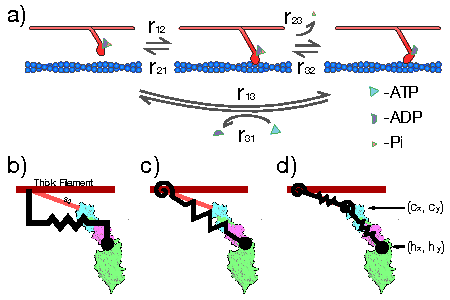
\includegraphics[width=3.2in]{../imgs/Figure1.pdf}
    \caption{
        \label{fig_xb_types}
        \textbf{Kinetic scheme and types of cross-bridges under investigation.} 
        The three state kinetic system is shown in subfigure A. 
        The three states represent (1) an unbound state, (2) a pre-power stroke state, and (3) a post-power stroke state. 
        The binding rate ($r_{1,2}$), power stroke rate ($r_{2,3}$), and unbinding rate ($r_{3,1}$) are determined by the energy stored in the springs representing the cross-bridge. 
        The reverse rates ($r_{2,1}$, $r_{3,2}$, and $r_{1,3}$) are functions of the forward transition rates and the energy stored in the cross-bridge in each state.
        Subfigures B, C, and D show the cross-bridge representations under consideration, plotted against a myosin crystal structure for comparison (structure image generated from \citet{Gourinath2003} with MacPyMol). 
        Subfigure B shows the single-spring cross-bridge (1sXB) introduced in \protect\citep{Huxley1957}. 
        Subfigure C depicts the two-spring cross-bridge (2sXB) which uses both a torsional/angular spring ($\theta$) and a linear spring ($\rho$). 
        Subfigure D shows the four-spring cross-bridge (4sXB) using two torsional and two linear springs. 
        The first torsional and linear spring of the 4sXB ($\alpha$ and $\beta$, respectively) correspond to the point at which the S2 region rejoins the thick filament backbone and the S2 region itself. 
        The second torsional and linear spring of the 4sXB ($\gamma$ and $\delta$, respectively) represent the area linking the S2 domain to the light chain domain and the light chain domain itself. 
It is $\gamma$, the second of the 4sXB's torsional springs, which replicates the change in angle at the converter domain accompanying the powerstroke.  
    }
    \end{center}
\end{figure}

\begin{figure}[ht]
    \begin{center}
    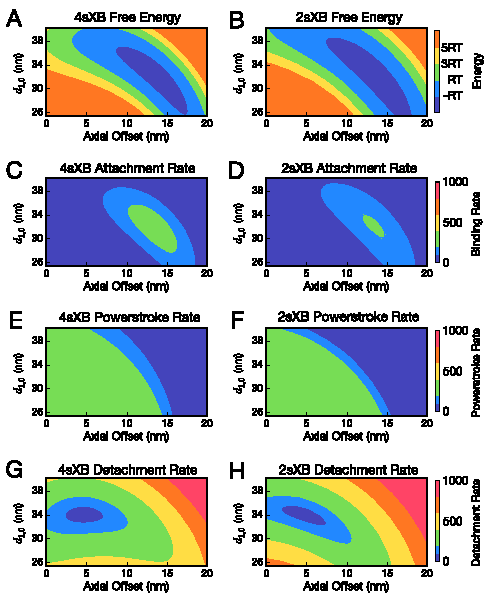
\includegraphics[width=3.2in]{../imgs/Figure2.pdf}
    \caption{
        \label{fig_kinetics_contours}
        \textbf{Energy and kinetics of the multi-spring cross-bridges as axial offset and lattice spacing change.} 
        Binding site offset is the distance between the current axial location of the cross-bridge's tip, $h_x$, and the location where the cross-bridge attaches to the thick filament.
        Lattice spacing ($d_{10}$) is defined as in \citet{Millman1998}, with an offset to account for filament thicknesses so that the cross-bridge bridges the two filaments at a rest lattice spacing of 34 nm.
        Subfigures A through H show the properties of the 4sXB (subfigures A, C, E, and G) and the 2sXB (subfigures B, D, F, and H) as they change with binding site offset and $d_{10}$ lattice spacing.
        Subfigure A depicts the free energy of the 4sXB at various lattice spacings (represented along the y-axis), with the head stretched to an axial offset from the thick filament attachment point (zero on the x-axis).
        Similarly, the free energy of the 2sXB is shown in subfigure B.
        The lowest energy myosin head locations in both A and B are shown as the darkest part of the plot and change in axial offset as lattice spacing changes.
        The subfigures C and D show $r_{1,2}$, the probability that the 4sXB and the 2sXB will transition from an unbound state to a bound state, and the dependence of this transition on both the axial offset of the open binding site from the myosin thick filament attachment site and the lattice spacing $d_{10}$ which is a function of the distance between the binding site and the thick filament attachment point of the myosin head. 
        Subfigure C depicts this probability for the 4sXB as a two dimensional contour with the same axes as in A while subfigure D depicts the transition probabilities for the two spring cross-bridge.
        Subfigures E and F show $r_{2,3}$, the probability of transition from a pre-power stroke state to a post-power stroke state, for the same cross-bridges, with the same axes and scales as C and D show $r_{1,2}$.
        Subfigures G and H show $r_{3,1}$, the probability of unbinding from a post-power stroke state, for the same cross-bridges, with the same axes and scales as C and D show $r_{1,2}$.
        The reverse rates, $r_{2,1}$, $r_{3,2}$, and $r_{1,3}$ are back-calculated from the forward rates.
    }
    \end{center}
\end{figure}

\begin{figure}[ht]
    \begin{center}
    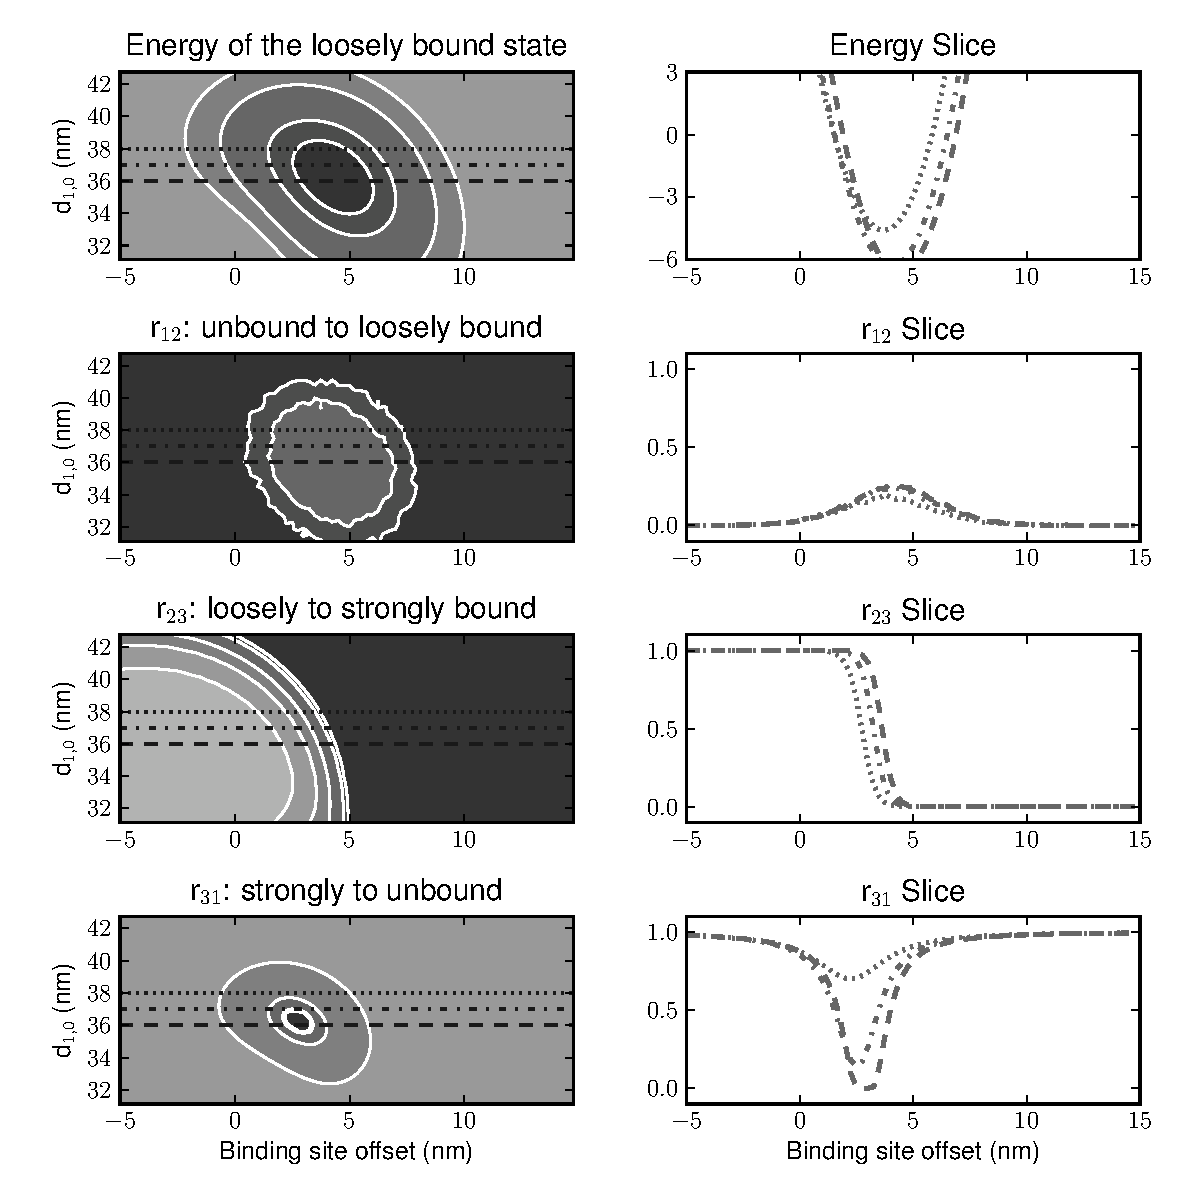
\includegraphics[width=3.2in]{../imgs/Figure3.pdf}
    \caption{
        \label{fig_kinetics_cuts}
        \textbf{Energy and kinetics of the 1sXB, 2sXB, and 4sXB at the resting lattice spacing.}
        Subfigures A through D show the energy and transition rates of the 1sXB (black), 2sXB (green), and 4sXB (red) at resting lattice spacing.
        The 1sXB values shown for comparison are derived from those of \citet{Daniel1998} and \citet{Tanner2007}, shifted axially so the resting location of the cross-bridge head in each case is aligned with the resting locations of the 2sXB and 4sXB\@. 
        The free energy of the cross-bridges in state two is shown in subfigure A, where the multi-spring cross-bridges' shifts from a strictly parabolic trajectory is visible.
        The explicit two-dimensional thermal forcing of the multi-spring cross-bridge heads in subfigure B results in binding probabilities that are more distributed than those of the single spring cross-bridge.
        The rate of power strokes, in subfigure C, remains least changed between the single and the multi-spring cross-bridge models.
        The energy-based kinetics of the multi-spring cross-bridges are unable to fully replicate the biased detachment rate of the 1sXB in subfigure D. 
    }
    \end{center}
\end{figure}

\begin{figure}[ht]
    \begin{center}
    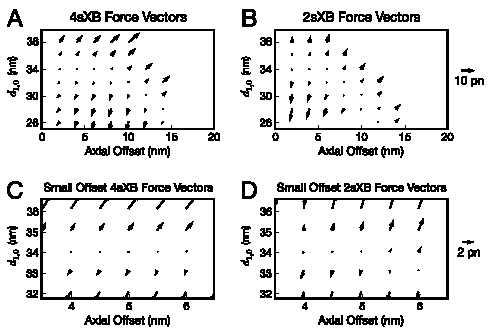
\includegraphics[width=3.2in]{../imgs/Figure4.pdf}
    \caption{
        \label{fig_forces}
        \textbf{Overview and detail of the forces exerted by the 2sXB and 4sXB\@.}
        Subfigures A through D show the forces exerted by the 4sXB and the 2sXB; omitted are vectors for unlikely configurations as determined by the sum of $r_{23}$ and the inverse of $r_{31}$. 
        Subfigures A and B show overviews of the forces exerted, respectively, by the 4sXB and the 2sXB over lattice spacings and axial offsets that vary as in Figure 2.
        The forces exerted by the two cross-bridges have radial components which frequently equal or exceed their axial components.
        A more detailed view of the region surrounding the rest position of the cross-bridges is shown in subfigures C and D, where the large radial components of the cross-bridge forces, particularly for the 2sXB, is again evident.
        Subfigures E through H show, separated, the axial and radial components of the 4sXB and the 2sXB\@.
    }
    \end{center}
\end{figure}

\begin{figure}[ht]
    \begin{center}
    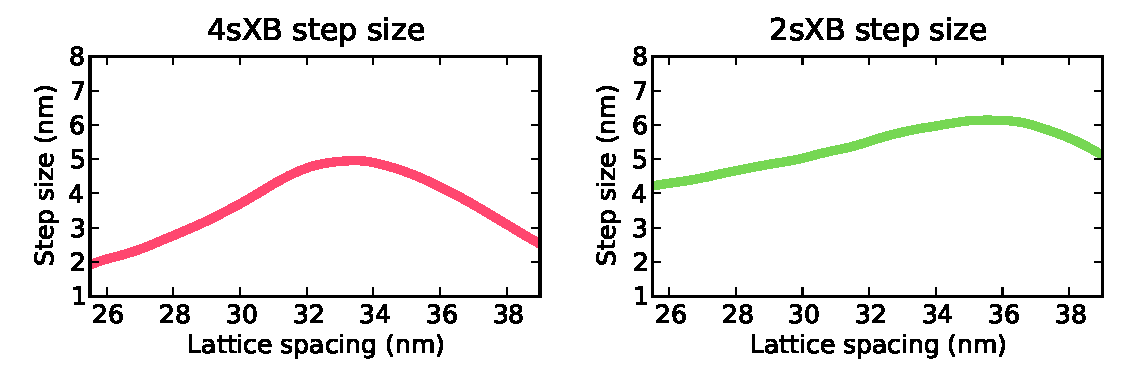
\includegraphics[width=3.2in]{../imgs/FigureS1.pdf}
    \caption{
        \label{fig_step_size}
        \textbf{Changes in step size with lattice spacing.}
    }
    \end{center}
\end{figure}

% bibliography (fold)
% Bib style requires biophysj.bst be in the document directory
\clearpage
\bibliographystyle{biophysj}
\bibliography{JournalArticles,NotArticles}
% bibliography (end)

\end{document}
